\chapter{The Simple Diagnostic Cloud Scheme}
\label{chp:simple_cld_scheme}

\section{Introduction}

As introduced in \chapref{ch:literature_review_about_clouds}, the cloud feedbacks have large uncertainty in

In order to have a cloud scheme that interacts with the radiation, we need to predict not only the cloud amount but also its radiative properties. We focus mainly on the former, for the latter we require effective radius of the cloud droplets, and in-cloud liquid water content. In the following subsections we describe how these are specified; an encapsulation of the cloud scheme is also given in \figref{fig:cld_scheme_summary}. 

\begin{figure}[t]
	\centering
	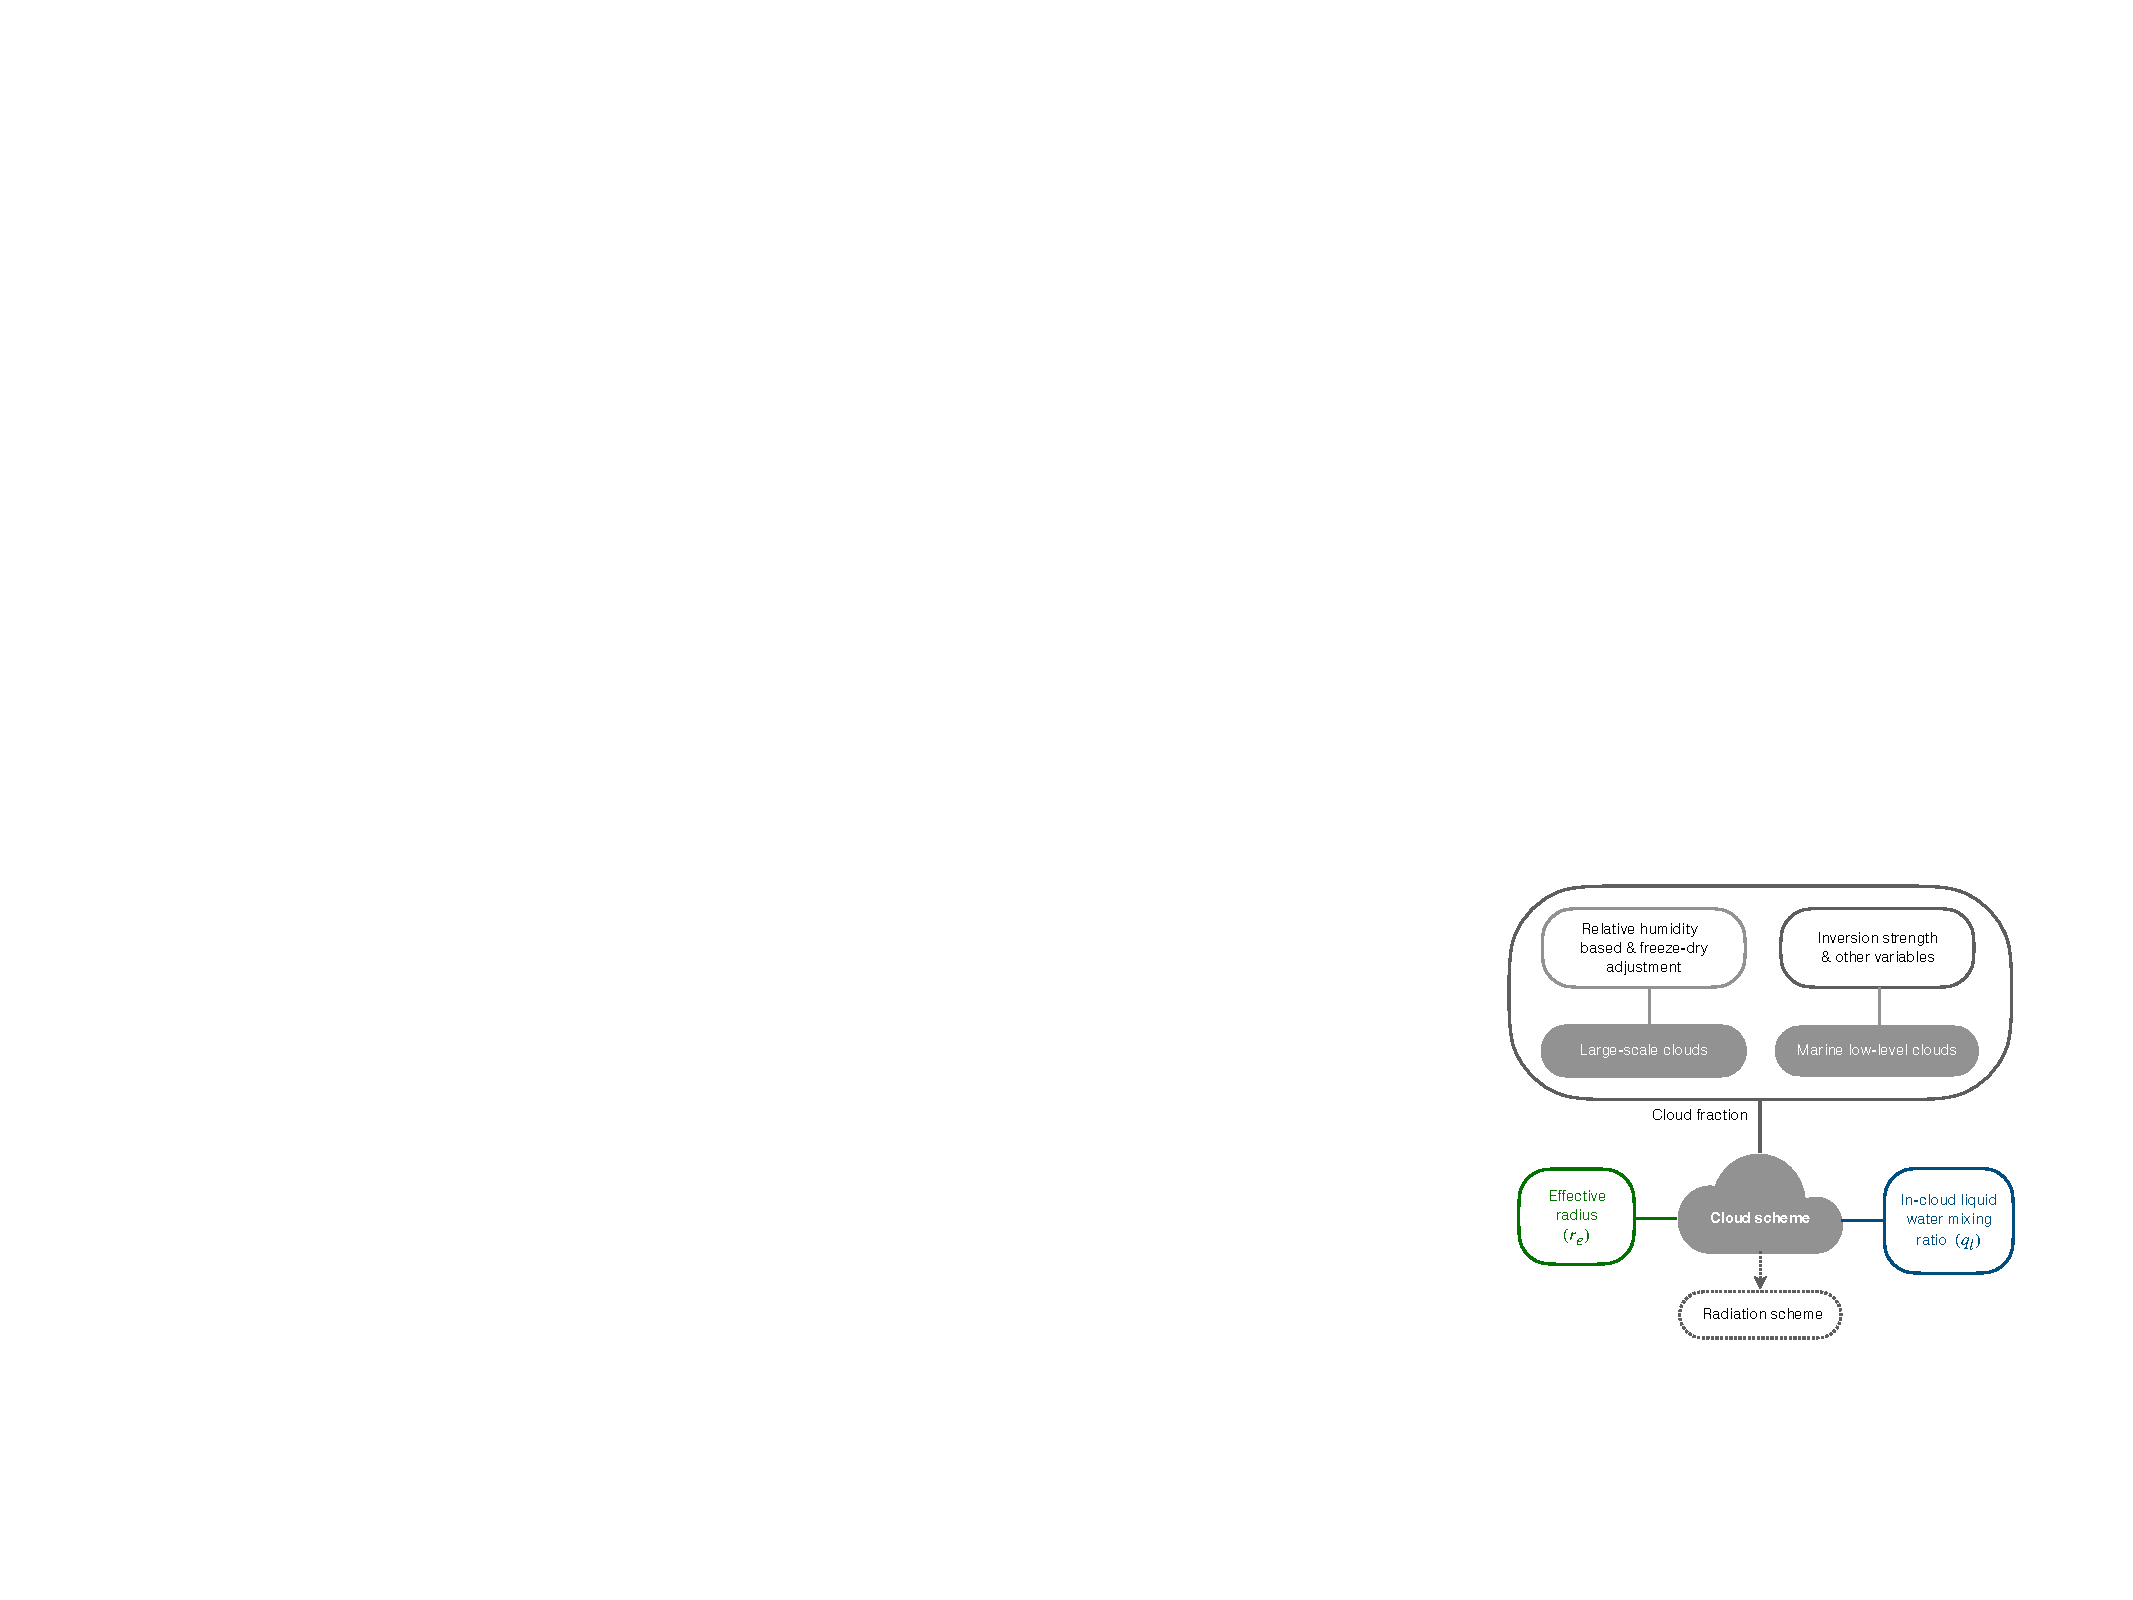
\includegraphics[width=0.7\linewidth]{figs/simple_cld_scheme/diag_cld_scheme_summary.pdf}
	\caption{A sketch of the simple cloud scheme components, which include the cloud fraction, effective radius of cloud droplet and in-cloud liquid water mixing ratio. At any given location, the maximum of the cloud fractions from large-scale cloud scheme and marine low stratocumulus cloud scheme is applied if both of them are used.} 
	\label{fig:cld_scheme_summary}
\end{figure}

%Clouds are represented in two ways in the scheme, `large-scale' clouds and low clouds. 
As noted in the introduction, large-scale clouds are parameterized as a function of relative humidity and this provides the majority of the cloud cover. However, as discussed in XXXXXXXXXXXXXXXXXX, this scheme alone is found to be inadequate and two additional effects are needed. First, a `freeze-dry' method based on the specific humidity is used to reduce the large-scale cloud cover over polar regions to more realistic levels. Second, a separate marine low stratus cloud scheme is used to represent the stratiform clouds (which have a large shortwave radiative effect), and this has a particularly large effect in subtropical regions off the west coast of continents. These two additional components are optional and users can decide whether to use according to their research interest. Although these clouds have different physical properties (e.g., cloud top temperature), all of them are treated essentially as liquid clouds in our scheme. The effective radius of the cloud droplets is allowed to change with temperature, and this affects the radiative transfer. Some tuning of the clouds scheme is performed in order to fit the observations. Nevertheless, the values of certain parameters used in the scheme are not necessarily definitive and may be varied in order to examine the sensitivity of clouds to perturbations such as CO$_2$ increase. 

The present version does not include a separate scheme for convective clouds, and the convection scheme in the model has no effect on cloudiness except in so far as it may change the relative humidity or, possibly, the low-level inversion.
%An alternative way to proceed would be to diagnose the convective clouds based on precipitation \citep[e.g.,][]{Gordon1992,Hack1998}, including that predicted by the convection scheme. 
We find that the vertical structure of clouds can be simulated relatively well without explicit diagnosis of convective clouds (see Figure..... \ref{fig:cld_fraction_profile}), and we leave the possible explicit representation of convective clouds to a future study. 


\section{Cloud fraction}

\subsection{Relative humidity-based cloud fraction}
\label{sec:rh_cloud}

The use of a relative humidity scheme is based on the notion that over a grid box the humidity varies, and that condensation will occur and clouds will form even when the grid cell is not saturated \citep{Tompkins2005, Quaas2012}, and one such scheme is that of \citet{Sundqvist1989}, discussed more below. Such schemes do not account for variations in dynamical conditions except in so far as they are reflected in the relative humidity field, but they form a simple rational basis for cloud prediction. Here we implement a large-scale cloud scheme in which the cloud fraction ($C_{s}$) is a piecewise linear function of grid-mean relative humidity ($H$), namely
\begin{equation}
	C_{s}=\min\left(1, ~\max \left(0, ~ a \cdot (H -1) + 1 \right)\right).
	\label{eq:linear_cf_rh} 
\end{equation}
The diagnosed cloud fraction is therefore unity when the mean relative humidity equal to one (i.e. grid-box is saturated). The value of $a$ determines the critical value of relative humidity, $H_c$, above which clouds form, so that $a=1/\left(1-H_{c}\right)$ and $H_c = (a -1)/a$. The coefficient $a$ (and hence $H_{c}$) is taken to be a function of height (or pressure) but not latitude or longitude. We also have implemented the \citet{Sundqvist1989} scheme, and that is available for users, but we do not describe it here. 

We derive the coefficient profile, the vertical values of the coefficient $a$, of the linear relationship between $C_s$ and relative humidity based on reanalysis data sets. Specifically, the hourly relative humidity and cloud fraction data sets in year 2017 from the European Centre for Medium-Range Weather Forecasts (ECMWF) Reanalysis version 5 (ERA5) \citep{era5} are used to derive the coefficient profile. Note that the saturated water vapor pressure is calculated over liquid and ice in ERA5 data set, while it is calculated over liquid only in the Isca simulations (see Sect.\ref{sec:exp_setup_and_dataset}). The ERA5 has $1^{\circ}\times 1^{\circ}$ horizontal resolution and 37 vertical levels. For each vertical level, the piecewise linear relationship (as cloud fraction is not allowed to be smaller than 0 or larger than 1) is used to fit the cloud fraction against relative humidity with a least squares method, then the coefficient $a$ of that level is obtained. In addition, data sets with three different horizontal resolutions, including $0.75^{\circ}\times 0.75^{\circ}$, $1.4^{\circ}\times 1.4^{\circ}$ (T85) and $2.8^{\circ}\times 2.8^{\circ}$ (T42), are used to test whether the derived coefficient profile is sensitive to horizontal resolution. The derived profiles with different resolutions are shown in \figref{fig:linear_coeff_profile}a, and the corresponding critical relative humidity ($H_c$) profiles are shown in \figref{fig:linear_coeff_profile}b for reference. At very high resolution we would expect the humidity distribution in a given grid box to be narrower, and hence the critical value of relative humidity to increase, however we find that the horizontal resolution has a relatively small influence on the coefficient profiles at the resolutions we consider here. 

To apply the coefficient profile of $a$ in the model, a profile similar to the Eq. (3) from \citet{Quaas2012} is used: %In addition, the global and regional data are also used to check whether the coefficient profiles would be different in various regions.
\begin{equation}
	a = a_t + (a_s-a_t)\exp{\left[1-\left( \frac{p_s}{p} \right)^{n} \right]},
	\label{eq:linear_coeff_a}
\end{equation}
where $p$ is the pressure, $p_s$ is the surface pressure, $a_s$ and $a_t$ are the values of coefficient $a$ at surface and free troposphere respectively. Such a functional form fits the observations fairly well with only a small number of tunable parameters. We use $a_s=36$, $a_t=13$ and $n=12$, which determines the shape of the profile. The fitted profile for $a$, as indicated by the solid pale blue line in \figref{fig:linear_coeff_profile}, follows the reanalysis (dashed/dotted lines) quite well at low and middle levels but with some discrepancies at higher levels. The actual cloud fraction for each level is determined by \Eqref{eq:linear_cf_rh}with the coefficient for that level determined by \Eqref{eq:linear_coeff_a}.

\begin{figure}
	\centering
	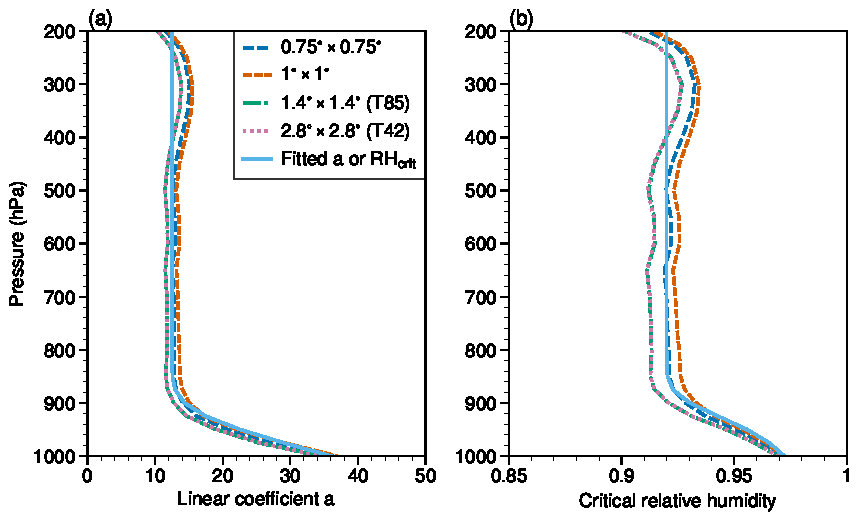
\includegraphics[width=0.8\textwidth]{{figs/simple_cld_scheme/fit_linear_coeff_profile}.pdf}
	\caption{(a) Vertical profiles of the linear coefficient for the relative humidity-based cloud diagnostic scheme, with cloud fraction as a piecewise linear function of relative humidity as shown in \Eqref{eq:linear_cf_rh}. The dashed lines with different colors are profiles of $a$ obtained from ERA5 data with various horizontal resolutions. The solid pale blue line denotes the fitted profile used in the model based on the form of \Eqref{eq:linear_coeff_a}. (b) is the same as (a), but for the critical relative humidity ($H_{c}$) profiles.}
	\label{fig:linear_coeff_profile}
\end{figure}

%To test the performance of this linear scheme, we also compare it with two other relative-humidity schemes. 
We also provide the \citet{Sundqvist1989} scheme as another option for the relative-humidity schemes, namely
\begin{equation}
	C_s = 1-\sqrt{\frac{1-H}{1-H_{c}}},
	\label{eq:sundqvist}
\end{equation}
where the $H_{c}$ is the critical relative humidity. Here we specify $H_{c}$ as a simple function of height, which is determined by critical relative humidity at three different levels: 0.95 at the surface, 0.85 at 700 hPa, and 0.99 at 200 hPa, which are determined
by running sensitivity tests. Between these levels, the critical relative humidity is linearly interpolated with height. To test the performance of the aforementioned schemes, we compare them with another linear scheme with different form from \Eqref{eq:linear_cf_rh}, which is defined as
% Second, we use another linear scheme with different form from \Eqref{eq:linear_cf_rh},
\begin{equation}
	C_s = \min\left(1, ~\max \left(0, ~ a \cdot H + b \right)\right),
	\label{eq:linear2}
\end{equation}
where $a$ and $b$ vary with height and are determined from the least squares fitting of hourly cloud fraction and relative humidity data from ERA5 reanalysis. The cloud fraction in \figref{fig:offline_cld_fraction_test}a is from ERA5 reanalysis at 450 hPa on 12:00 January 01, 2017, while the cloud fractions from three schemes (\figsref{fig:offline_cld_fraction_test}b-\ref{fig:offline_cld_fraction_test}d) are diagnosed from the ERA5 relative humidity field at the same time and level. The linear scheme defined in \Eqref{eq:linear2} has two tunable parameters, so one might expect it to perform better than the others. However, the cloud cover can not reach 1 when the grid box is saturated (\figref{fig:offline_cld_fraction_test}c), even though the spatial pattern of cloud cover resembles the ERA5 reanalysis and the global mean value is much closer to the ERA5 compared to the other two schemes. In contrast, the diagnosed cloud amount patterns from Sundqvist scheme (\figref{fig:offline_cld_fraction_test}b) and the linear scheme in the form of \Eqref{eq:linear_cf_rh} (\figref{fig:offline_cld_fraction_test}d) are quite similar to the reanalysis (\figref{fig:offline_cld_fraction_test}a), although the cloud cover is a little overestimated in these two schemes. These offline tests suggest that the linear scheme in the form of \Eqref{eq:linear_cf_rh} is promising to be applied in GCMs.

\begin{figure}
	\centering
	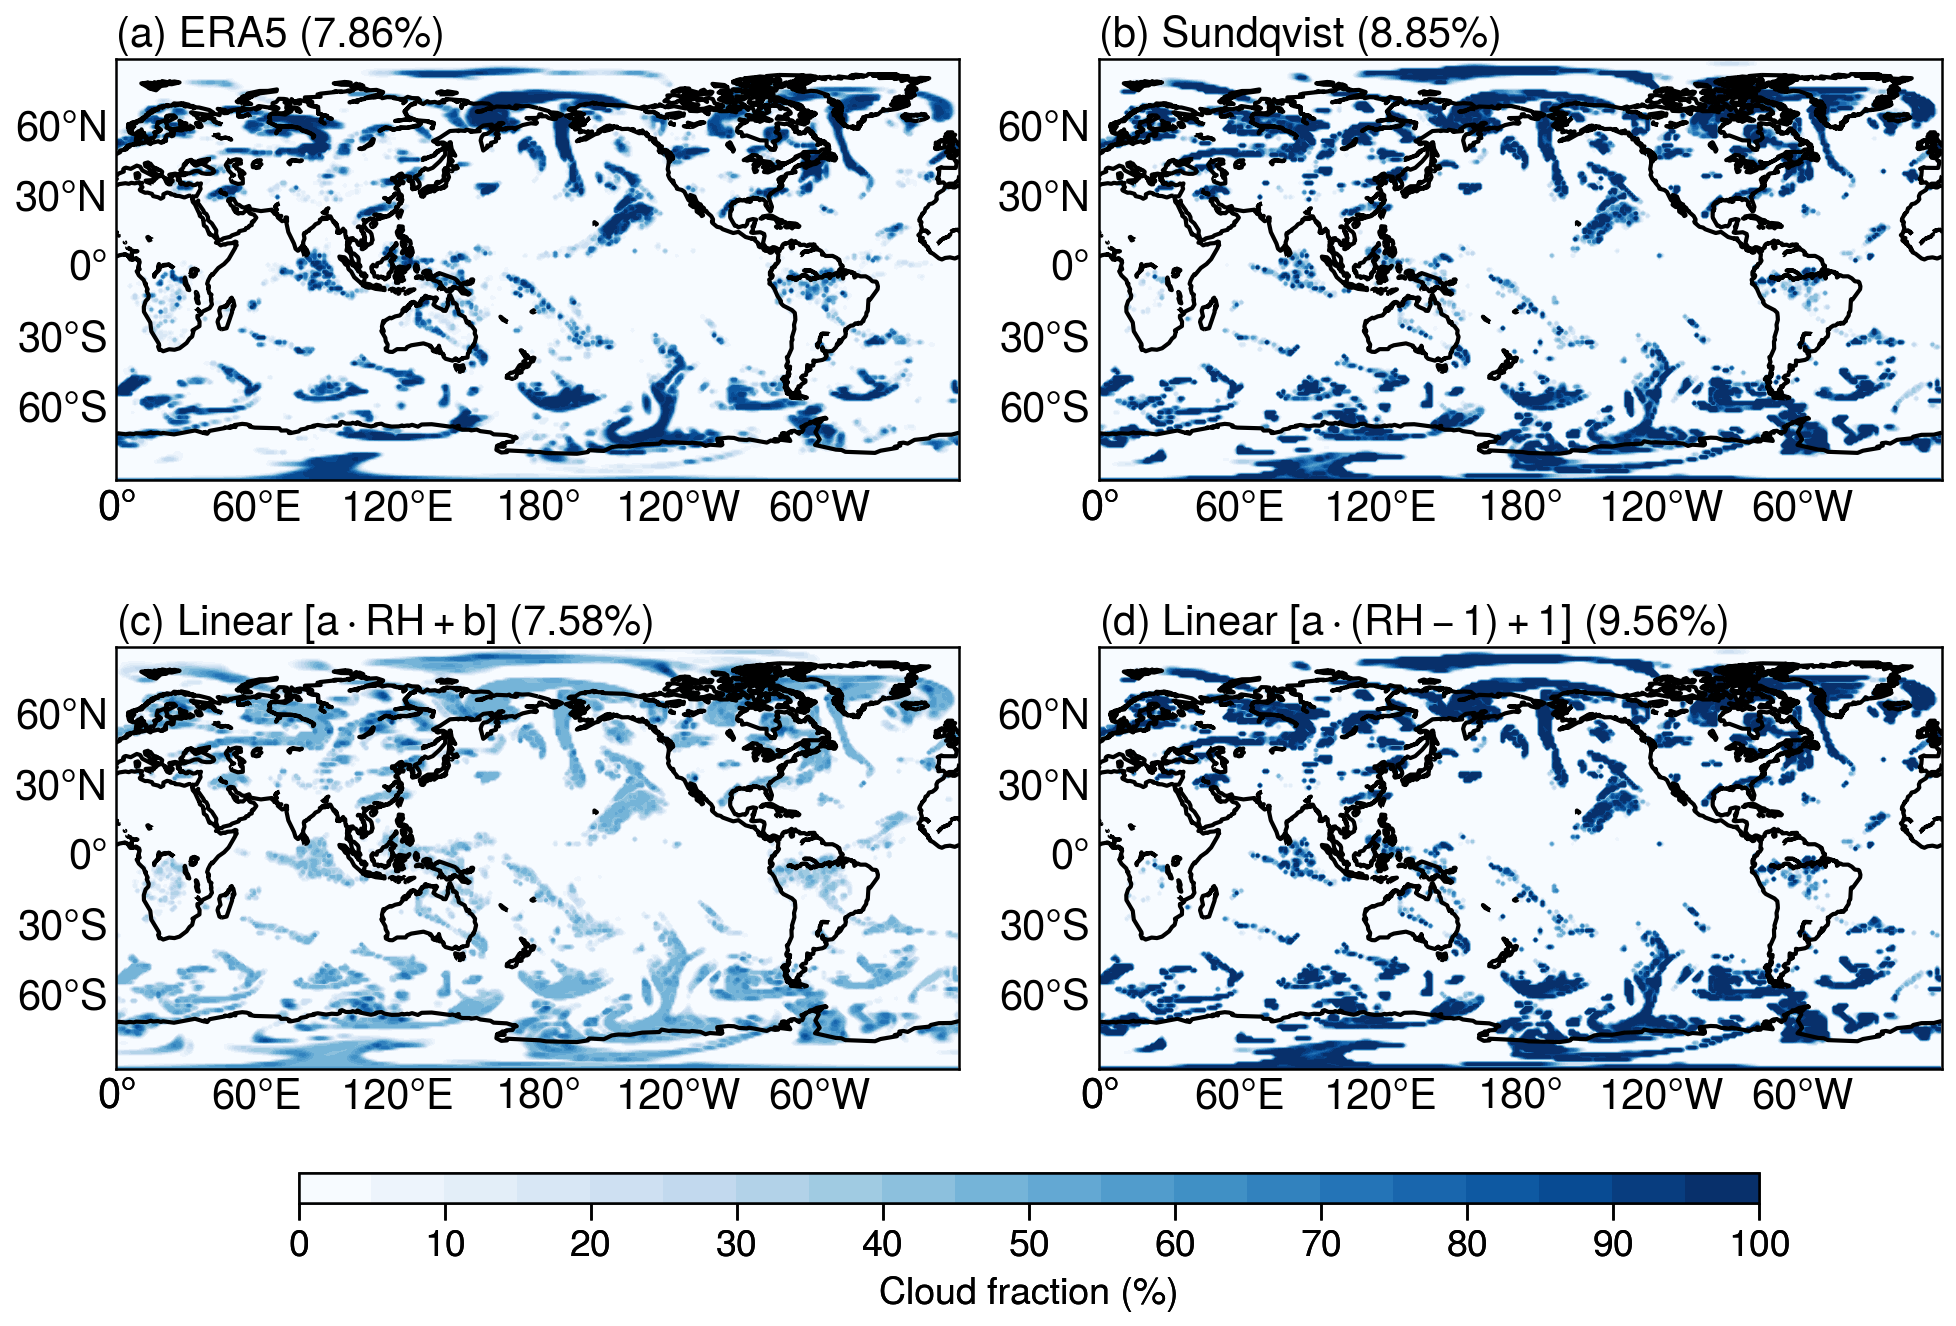
\includegraphics[width=1\linewidth]{{figs/simple_cld_scheme/cmp_sundqvist_linear_with_ecmwf_cc_t_12_lev_20}.png}
	\caption{(a) A snapshot of cloud fraction from ERA5 reanalysis at 450 hPa on 12:00 January 01, 2017. Diagnosed cloud fraction from ERA5 relative humidity field at the same time and level based on the (b) Sundqvist formula, and two linear formulas (c) using \Eqref{eq:linear2} and (d) using \Eqref{eq:linear_cf_rh}. Note that \Eqref{eq:linear_cf_rh} is the form used to determine the large-scale clouds in this study. The global mean cloud fractions are given in the titles.} 
	% [$\min\left(1, ~\max \left(0, ~ a \cdot H + b \right)\right)$],  [i.e., $\min\left(1, ~\max \left(0, ~ a \cdot (H -1) + 1 \right)\right)$]
	\label{fig:offline_cld_fraction_test}
\end{figure}

\subsection{Freeze-dry adjustment}
\label{sec:freezedry}

As we will show in \secref{sec:cld_amt}, the cloud fraction and LW cloud radiative effect from the large scale cloud scheme are overestimated in polar regions, especially during winter. The relative humidity-based cloud fraction scheme assumes there are subgrid-scale fluctuations of humidity and/or temperature, so the partial cloudiness is possible even under subsaturated conditions averaged over a grid box. However, this assumption might not be well suited for the extremely cold and dry atmospheric conditions in polar winter \citep{Jones2004}. The stable boundary layer condition in polar winter leads to little subgrid-scale spatial variability in humidity fields, and there should be less cloudiness than the turbulent environment for a given relative humidity. To alleviate this problem we implement a `freeze-dry' adjustment, a simple adjustment formula based on specific humidity from \citet{Vavrus2008} (see their Eq. (2)). The freeze-dry adjustment is applied to reduce the cloud fraction under very dry conditions in polar regions. Specifically, if grid mean specific humidity ($q$) is below a threshold ($q_v$), the cloud fraction ($C$) decreases linearly according to the water vapor content:
\begin{equation}
	C= C\cdot f=C \times \max \left(0.15, \min \left(1.0, ~\frac{q}{q_{v}}\right)\right),
	\label{eq:freeze-dry}
\end{equation}
in which the second term is called the freeze-dry factor ($f$). Although the formula is applied globally, the threshold value in \Eqref{eq:freeze-dry} ensures that only polar regions will be affected and even there the cloud fraction is adjusted only under very dry conditions.

\begin{figure}[ht]
	\centering
	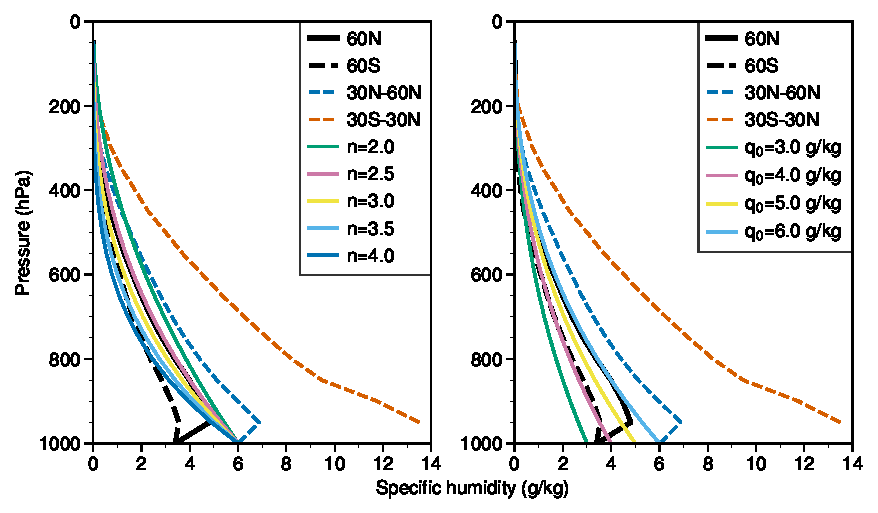
\includegraphics[width=1\linewidth]{{figs/simple_cld_scheme/feezedry_with_various_qv}.pdf}
	\caption[The $q_v$ vertical profiles with different $n$ and $q_0$.]{The $q_v$ vertical profiles with different $n$ and $q_0$. The thick solid and dashed black lines are annual mean specific humidity profiles from Isca simulation averaged over latitude circles, 60N and 60S, as boundary values of polar regions in Northern and Southern hemispheres, respectively. The thin dashed blue and orange lines are averaged specific humidity profiles over subtropical (30$^\circ$-60$^\circ$N) and tropical (30$^\circ$S-30$^\circ$N) regions in Isca simulation. The remaining solid lines are from \Eqref{eq:qv_freeze-dry} with different parameters. In the left, $q_0$ in \Eqref{eq:qv_freeze-dry} is 0.006 kg kg$^{-1}$ but $n$ varies from 2 to 4. In the right, $n=2.5$ but $q_0$ varies from 0.003 to 0.006 kg kg$^{-1}$.} 
	% The thick solid and dashed black lines, and the thin dashed blue and orange lines are averaged specific humidity profiles from different regions in Isca simulation. 
	\label{fig:freeze-dry}
\end{figure}

In the original freeze-dry method, \Eqref{eq:freeze-dry} was only applied in the lower troposphere \citep{Vavrus2008}. In this study, the freeze-dry formula is applied through the whole atmospheric column, finding that the cloud radiative effect in polar regions is thereby improved. In order to do so, we prescribe the specific humidity threshold $q_v$ in \Eqref{eq:freeze-dry} to be a function of pressure with the threshold decreasing exponentially with height as
\begin{equation}
	q_{v} = q_0\left(\frac{p}{p_s}\right)^n.
	\label{eq:qv_freeze-dry}
\end{equation}
Here $q_0$ is the surface specific humidity, $p_s$ is the sea level pressure ($p_s=1000$ hPa) and $n$ is the power to describe how quickly the specific humidity decreases with height. In \figref{fig:freeze-dry}, different profiles of $q_v$ are shown for the two tunable parameters $n$ and $q_0$. These two parameters are selected to ensure that the freeze-dry adjustment only has effects on polar regions when the $q_v$ profile is applied in \Eqref{eq:freeze-dry}. In doing so, the specific humidity profiles from several different regions are plotted in \figref{fig:freeze-dry}. In particular, the profiles at $60^{\circ}$N and $60^{\circ}$S are used to show the specific humidity boundary values of polar regions, and thus the two parameters $q_0$ and $n$ are tuned to follow the boundary profiles. As shown in \figref{fig:freeze-dry}, the $q_v$ profile follows the $60^{\circ}$N profile well when the $q_0=0.006$ kg kg$^{-1}$ and $n=2.5$, which can also cover the specific humidity range poleward of $60^{\circ}$S. Therefore in this study the parameters $q_0$ and $n$ are chosen as 0.006 kg kg$^{-1}$ and 2.5, respectively. This threshold works well in current climate setup (see \secref{sec:cld_amt}), but whether it holds under global warming situation still needs further investigation.


\subsection{Low cloud fraction}

Low clouds, especially the subtropical marine stratocumulus clouds, are characterized by high albedo and a cooling effect on climate \citep{Hartmann1992}. Because these clouds cover about 20\% of the subtropical regions even a small change in stratocumulus cloud amount can exert a large radiative forcing at the top of the atmosphere (TOA) \citep{Slingo1990}. However, marine stratocumulus amounts off the west coast of continents have commonly been underestimated and has been an issue in climate models for some time \citep[e.g.,][]{Nam2012, Lauer2013, Dolinar2015}.

Several proxies or indices for low cloud fraction have been used as predictors for the stratocumulus clouds to try to remedy this \citep[e.g.,][]{Kawai2006, Joshi2015, Collins2004, Guo2014, Kawai2019}, including potential temperature lapse rate ($d\theta/dp$) of the most stable layer below 750hPa \citep{Slingo1987}; lower tropospheric stability \citep[LTS;][]{Klein1993}; estimated inversion strength \citep[EIS;][]{Wood2006}; and the estimated cloud-top entrainment index \citep[ECTEI;][]{Kawai2017}. Recently, \citet{Park2019} proposed a new index, the estimated low-level cloud fraction (ELF), as a predictor for low cloud fraction. ELF (which is a proxy and not necessarily a cloud amount itself) is defined as
%, denoted $\ELF$
\begin{equation}
	\text{ELF} \equiv f \cdot\left[1-\frac{\sqrt{z_{inv} \cdot z_{LCL}}}{\Delta z_{s}}\right],
	\label{eq:ELF}
\end{equation}
where $f$ is the freeze-dry factor defined in \Eqref{eq:freeze-dry} with $q_v=0.003$ kg kg$^{-1}$ and $q$ is the surface water vapor specific humidity,  $z_{inv}$ is the inversion height, $z_{LCL}$ is the lifting condensation level of near-surface air, and $\Delta z_{s}$ is a constant scale height ($\Delta z_{s}= 2750$m). As pointed by \citet{Park2019},
$\sqrt{z_{inv} \cdot z_{LCL}}/\Delta z_{s}$ can be rewritten as $z_{LCL}/\Delta z_{s}\cdot \sqrt{1+(z_{inv} -z_{LCL})/z_{LCL}}$, in which $z_{LCL}/\Delta z_{s}$ is a simple but practical proxy of surface moisture, and $(z_{inv}-z_{LCL})/z_{LCL}$ quantifies the strength of the vertical decoupling of the inversion base air from the surface. The ELF predicts that low-level cloud fraction increases as the near-surface air gets more wet (smaller $z_{LCL}$) and as the planetary boundary layer becomes more vertically coupled (smaller $z_{inv}$).

\begin{figure}[ht]
	\centering
	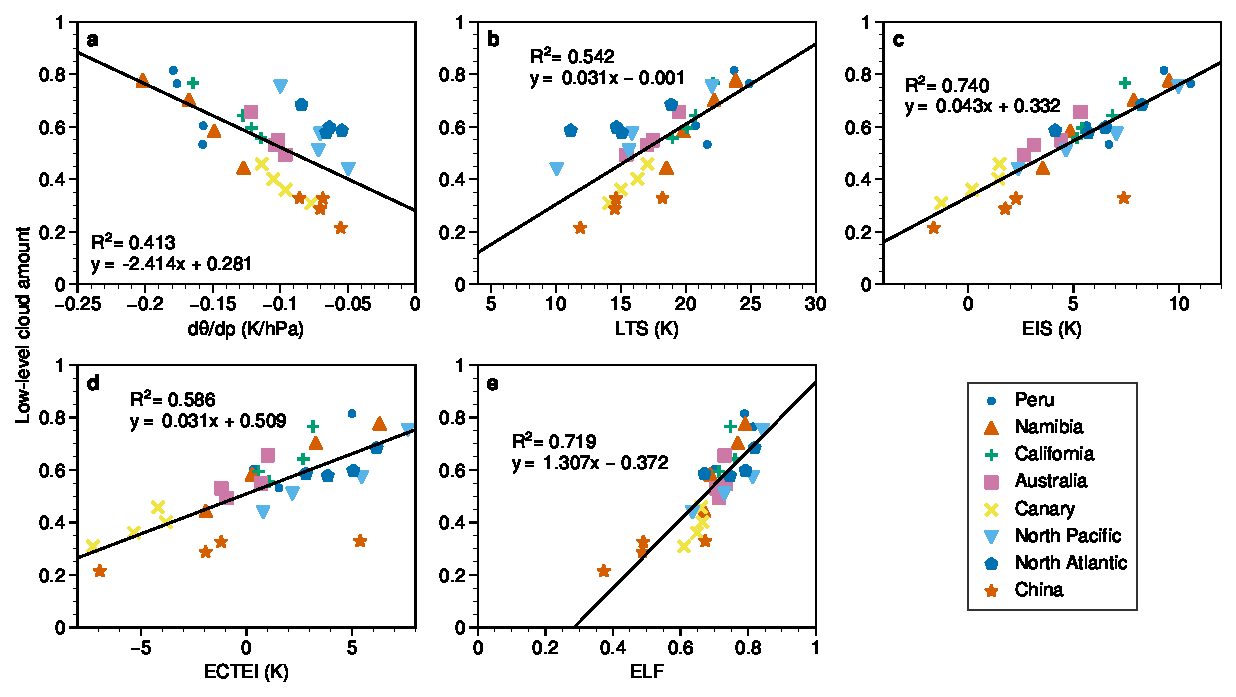
\includegraphics[width=1\linewidth]{{figs/simple_cld_scheme/low_cld_frac_vs_diff_vars_season}.pdf}
	\caption[The relationship between low-level cloud amount and proxies.]{The relationship between low-level cloud amount and (a) minimum $d\theta/dp$ below 750 hPa, (b) lower tropospheric stability (LTS), (c) estimated inversion strength (EIS), (d) estimated cloud-top entrainment index (ECTEI) and (e) estimated low cloud fraction (ELF) over stratiform cloud regions, including Peru (20$^\circ$S-5$^\circ$N, 80$^\circ$-90$^\circ$W), Namibia (10$^\circ$-30$^\circ$S, 0$^\circ$-15$^\circ$E), California (15$^\circ$-30$^\circ$N, 110$^\circ$-150$^\circ$W), Australia (15$^\circ$-35$^\circ$S, 90$^\circ$-110$^\circ$E), Canary (15$^\circ$-25$^\circ$N, 25$^\circ$-35$^\circ$W), North Pacific (40$^\circ$-5$^\circ$0N, 170$^\circ$-180$^\circ$E), North Atlantic (50$^\circ$-60$^\circ$N, 35$^\circ$-45$^\circ$W) and China (20$^\circ$-30$^\circ$N, 105$^\circ$-120$^\circ$E), which are selected based on \citet{Klein1993}. The data sets are from ERA-Interim reanalysis covering the period from 2013 to 2017. The four points in each region denote the average for different seasons. Linear regression lines and the corresponding fraction of variance ($R^2$) explained by the equation are shown at the top of each plot.}
	\label{fig:fit_low_cld_proxy}
\end{figure}

We have examined the relationship between the seasonal mean low cloud fraction and the various proxies (i.e., $d\theta/dp$, LTS, EIS, ECTEI and ELF) using the ERA-Interim reanalysis data set \citep{Dee2011}. These proxies are derived from the five-year monthly data from 2013 to 2017, including air temperature, surface pressure, surface temperature and low cloud fraction. As shown in \figref{fig:fit_low_cld_proxy}, the regions with typical stratus clouds are selected for the calculation \citep{Klein1993}. The results indicate that the low cloud fraction is linearly related to each indicator in stratus clouds regions, and the ELF tends to have very high correlation with the low-level cloud cover, judging from the fraction of variance ($R^2$) explained by the regression equation. We thus choose to use ELF to construct the diagnostic low cloud fraction formula, that is:
\begin{equation}
	C_{sc} = \min(1, ~\max(0, ~b\times \text{ELF} + c)),
	\label{eq:sc_ELF}
\end{equation}
where $C_{sc}$ is the low stratus cloud fraction, and the two coefficients $b$ and $c$ are treated as tunable parameters. The linear regression formula displayed in \figref{fig:fit_low_cld_proxy}e provides a good starting point for tuning $b$ and $c$ in \Eqref{eq:sc_ELF}. After a sensitivity test performed with Isca (the setups will be introduced in \secref{sec:exp_setup_and_dataset}), we find that if $c$ is specified as the value shown in \figref{fig:fit_low_cld_proxy}e, the shortwave cloud radiative effect is still weak compared to observations. Therefore the parameters $b$ and $c$ are chosen as 1.3 and -0.1 respectively.

In addition, the stratocumulus clouds usually form at the top of planetary boundary layer \citep{Wood2012}, where a strong inversion layer usually exists \citep{Wood2006,Park2019}. However, it is hard for a global model to capture the exact position of the inversion layer due to the limitation of vertical resolution \citep{Kawai2019}. Care thus needs to be taken to diagnose the marine stratocumulus clouds. First we find the most stable layer below 750 hPa, which is determined by the most negative $d\theta/dp$ \citep{Slingo1987}. Then within the most stable layer, if the lapse rate and vertical velocity satisfy $d\theta/dp<-0.08$ K hPa$^{-1}$ and $\omega>0$ Pa s$^{-1}$ respectively, then we diagnose stratocumulus clouds at that location. Note that the $d\theta/dp$ threshold is tuneable in our scheme, and it is $-0.125$ K hPa$^{-1}$, as in \citet{Collins2004}.

\subsection{Cloud fraction diagnosis}
\label{sec:cld_amt_diag}

The cloud fraction of a grid box ($C_\mathrm{total}$) is simply defined as the largest fraction of all the clouds within that grid box for simplicity, without separate consideration of their different optical properties:
\begin{equation}
	C_\mathrm{total}=\max(C_s, ~C_{sc}),
	\label{eq:CF_total}
\end{equation}
assuming a horizontal maximum overlap hypothesis \citep[e.g.,][]{Collins2004, Roehrig2020}. $C_s$ and $C_{sc}$ in \Eqref{eq:CF_total} are determined by \Eqref{eq:linear_cf_rh} and \Eqref{eq:sc_ELF} respectively. To assess the performance of the cloud scheme, it is useful to evaluate the total cloud amount and cloud amounts at different levels. In our scheme, the cloud height is determined by cloud top pressures, where those located above 400 hPa are treated as high clouds, those below 700 hPa are defined as low clouds, and in between are middle clouds \citep{Collins2004}. Then, the total, high, middle or low cloud amounts are diagnosed from the maximum-random overlap assumption \citep{Morcrette2000}, which assumes maximum overlap for consecutive cloudy model levels and random overlap for cloud layers that are separated by clear-sky levels.

\section{Effective radius}

Cloud particles, including liquid droplets and ice crystals, usually have different sizes, shapes and optical properties. In order not to introduce complicated microphysical processes, we do not distinguish them and assume that all particles seen by the radiation scheme are spherical liquid droplets, and ice clouds have a different effective radius from the liquid ones. In this study, the liquid cloud fraction varies with temperature, which only has an influence on the effective radius. %and ice clouds have a different effective radius from liquid ones.

Following \citet{Ose1993} and \citet{Boville2006}, a very simple approach is used to represent the liquid cloud fraction ($f_l$) within a grid box. Specifically, all clouds are assumed to be in liquid form if temperature is warmer than $T_{max}$, and all the condensate is considered as ice if temperature is colder than $T_{min}$. The cloud droplets are in mixed-phase at temperatures between $T_{min}$ and $T_{max}$, and the proportion of liquid cloud in a grid box is defined as a linear function of temperature:
\begin{equation}
	f_{l} =\max\left(0, ~\min\left(1, ~\frac{T-T_{min}}{T_{max}-T_{min}} \right)\right).
	\label{eq:liquid_frac}
\end{equation}
The bounds $T_{min}$ and $T_{max}$ are different in different models. For example, the lower bound ($T_{min}$) is $-40^{\circ}$C in \citet{Ose1993} and \citet{Boville2006}, while it is $-15^{\circ}$C  in \citet{Smith1990}. Observations have shown that cloud liquid water can exist at temperature as low as $-40^{\circ}$C \citep{Heymsfield1993}, although the incidence of liquid water in stratiform clouds is quite low at temperatures below $-15^{\circ}$C \citep{Ryan1996}. The upper bounds ($T_{max}$) are $-5^{\circ}$C for stratiform clouds in \citet{Ose1993}, $-10^{\circ}$C in \citet{Boville2006}, and $0^{\circ}$C in \citet{Smith1990}. Based on the choices in previous studies, $T_{min}$ and $T_{max}$ in \Eqref{eq:liquid_frac} are chosen to use $-40^{\circ}$C and $-5^{\circ}$C respectively in this study, but they are to be regarded as adjustable parameters.

The effective radius ($r_{e}$) of droplets within a grid box is defined as a weighted mean of liquid and ice particle radii, with the weights given by the liquid and ice cloud fraction respectively. The radii of liquid and ice particles are selected based on observations. \citet{Stubenrauch2013} assessed cloud properties derived from various satellite data sets, finding that the global mean effective particle radii are about $14$ ($\pm1$) and $25$ ($\pm2$) $\mu m$ for the tops of liquid clouds and for high-level ice clouds, respectively. Therefore these two values are selected to calculate $r_e$,
\begin{equation}
	r_e = 14f_l + 25(1-f_l),
	\label{eq:Reff}
\end{equation}
which is applied globally in the model, although the effective radius of cloud droplets is found a little larger over ocean than over continents in observations \citep{Stubenrauch2013}.

\section{In-cloud water mixing ratio}

The in-cloud liquid water mixing ratio ($q_l$) is specified as a linear function of the atmospheric temperature, with values of $3\times 10^{-4}$ g kg$^{-1}$ at $220$ K and $q_{l0}=0.18$ g kg$^{-1}$ at $280$ K:
\begin{equation}
	w_l = \max\left(3\times 10^{-4}, ~w_{l0}\times  \min\left(1, ~\frac{T-220}{280-220}\right)\right),
	\label{eq:qcl}
\end{equation}
where the atmospheric temperature $T$ is in units of K. The temperature thresholds, 280 and 220 K, are selected close to the global averages of liquid and ice cloud top temperature in observations, respectively \citep[Fig. 4 in][]{Stubenrauch2013}. Then the grid mean liquid water specific humidity can be obtained from the product of $w_l$ and cloud fraction. Note that \Eqref{eq:qcl} is modified from the SPOOKIE II project (see \url{https://www.cfmip.org/experiments/informal-experiments} for detail). At first, the in-cloud water content is specified as a function of height, but in the second version of the protocol, it has been updated as a function of temperature.

\section{Summary and discussions}

This chapter presents how the simple cloud scheme was build. For reference, the equations and parameters used in the cloud scheme are summarized in Table \ref{tab:cld_scheme_summary}. 

\begin{sidewaystable}
	\caption{Summary of the diagnostic cloud scheme.}
	\vspace{0.5em}
	\centering
	\renewcommand{\arraystretch}{1.5}
	\begin{tabular}{c c p{6cm} p{7cm} l} 
		\toprule
			\multirow{2}{*}{Symbol} & Range  & \multirow{2}{*}{Definition} & \multirow{2}{*}{Diagnostic formula} & \multirow{2}{*}{Tunable parameters} \\
			& / Units & & & \\
			\hline
			\multirow{3}{*}{$C_s$} & \multirow{3}{*}{[0, 1]} & \multirow{3}{*}{Large-scale cloud fraction} & $\min\left(1, ~\max \left(0, ~a \cdot (H-1) + 1 \right)\right)$,&  \multirow{2}{*}{$a_s$=36, $a_t$=13, $n$=12} \\
			& &  &	$a=a_t + (a_s-a_t)\exp{\left[1-\left( \frac{p_s}{p} \right)^{n} \right]}$& \\ \cline{4-5}
			& &  &	$\min\left(1, ~\max \left(0, ~1-\sqrt{\frac{1-H}{1-H_{c}}} \right)\right)$ & $H_c$: function of height  \\
			\hline
			\multirow{2}{*}{$f$}  & \multirow{2}{*}{[0.15, 1]} & \multirow{2}{*}{Freeze-dry adjustment factor} & $\max \left(0.15, \min \left(1.0, ~\frac{q}{q_{v}}\right)\right)$, & \multirow{2}{*}{$q_0$=6 g kg$^{-1}$, $n$=2.5} \\
			& & & $q_{v}= q_0\left(\frac{p}{p_s}\right)^n$ & \\
			\hline 
			\multirow{2}{*}{$C_{sc}$} & \multirow{2}{*}{[0, 1]} & \multirow{2}{*}{Low cloud fraction} & $\min(1, ~\max(0, ~b\times \text{ELF} +c))$, & $b$=$1.3$, $c$= $-0.1$  \\
			& & &  $\text{ELF}=f \cdot\left[1-\sqrt{z_{inv} \cdot z_{LCL}}/{\Delta z_{s}}\right]$  & $q_v$=3 g kg$^{-1}$ in $f$ \\
			\hline 
			\multirow{2}{*}{$f_l$} & \multirow{2}{*}{[0, 1]}  & \multirow{2}{*}{Liquid cloud fraction} & $\max\left(0, ~\min\left(1, ~\frac{T-T_{min}}{T_{max}-T_{min}} \right)\right)$, & \multirow{2}{*}{$T_{min}$=$-40$, $T_{max}$=$-5$$^\circ$C} \\
			& & & ($T$ in units of $^\circ$C) & \\
			\multirow{2}{*}{$r_e$} & [$r_{e\_liq}$, $r_{e\_ice}$] & \multirow{2}{*}{Effective radius} & \multirow{2}{*}{$r_{e\_liq}f_l + r_{e\_ice}(1-f_l)$} & \multirow{2}{*}{$r_{e\_liq}$=14, $r_{e\_ice}$=25 $\mu$m} \\
			&  $\mu$m & & & \\
			\hline
			\multirow{2}{*}{$w_l$} & [$3\times 10^{-4}$, $w_{l0}$] & \multirow{2}{*}{In-cloud liquid water mixing ratio} & $\max\left(3\times 10^{-4}, ~w_{l0}\times \min\left(1, ~\frac{T-220}{280-220}\right)\right)$,& \multirow{2}{*}{$w_{l0}$=0.18 g kg$^{-1}$} \\
			& g kg$^{-1}$ & & ($T$ in units of K)  & \\
		\bottomrule
	\end{tabular}
	\label{tab:cld_scheme_summary}
\end{sidewaystable}
